% !TeX root = ..//diffgeo_main.tex
\begin{satz}[$(\mfk, \dd)$ als metrischer Raum]
\label{satz:metrischer_raum}
$(\mfk, \dd)$ ist ein metrischer Raum, das bedeutet:
\begin{enumerate}
\item  $\dd(p, q) = \dd(q, p)$
\item  $\dd(p, q) = 0  \quad \Leftrightarrow \quad p=q$
\item  $\dd(p, q) \leq \dd(p, r) + \dd(r, q)$
\end{enumerate}
Außerdem ist $\dd: \mfk \rightarrow \mfk$ stetig und die von $\dd$ induzierte Topologie ist die ursprüngliche Topologie auf $\mfk$.
\end{satz}
Für den Beweis des Satzes benötigen wir ein Hilfslemma.
\begin{lem}
Sei $\varepsilon>0$ und $B_{\varepsilon}(0) = \{ v \in T_p\mfk | \norm{v} < \varepsilon\} \subseteq T_p\mfk$. Sei außerdem $\varepsilon$ klein genug, so dass $\eval{\expp_p}_{B_{\varepsilon}(0)}$ ein Diffeomorphismus ist. Setze $B_{\varepsilon}(p) = \expp_p(B_{\varepsilon}(o)) \subseteq \mfk$.
\begin{enumerate}
\item Dann ist $\forall v \in B_{\varepsilon}(0)$ die Geodätische $c_v$ die bis auf Umparametrisierungen eindeutige, kürzeste Verbindung von $p$ nach $q=\expp_p(v)$.
\item Sei $q \notin B_{\varepsilon}(p)$. Dann gilt für jede Kurve $c$ von $p$ nach $q$: $L(c) < \varepsilon$.
\end{enumerate}
\begin{figure}[H]
	\centering
	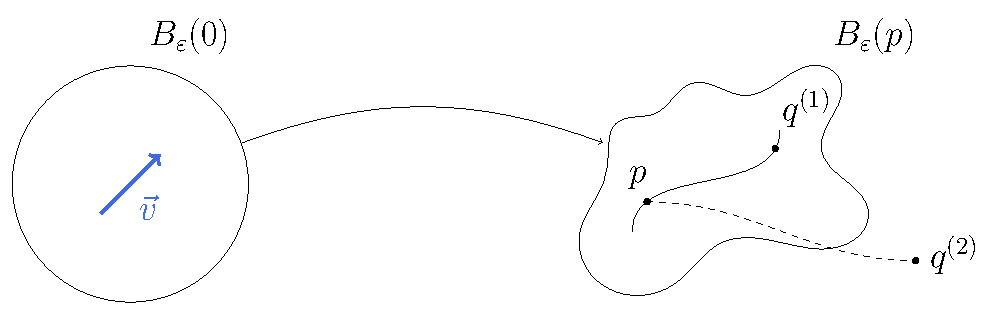
\includegraphics[scale=0.65]{figures/tikz/lemma_geodesics}
	\caption{Graphische Darstellung der zweiten Aussage des Lemmas}
\end{figure}
\end{lem}
\begin{bew}
Sei $c:[a, b] \longrightarrow \mfk$ Kurve mit $c(a)=p$ ud $c(b)=q=\expp_p(v)$ wobei für das Bild von $c$ gilt: $\operatorname{Im}(c) \subset B_{\varepsilon}(p)$. Setze:
\begin{align*}
\bar{c}(t) &= \expp_p^{-1}(c(t)) \\
s(t) &= \norm{\bar{c}(t)} \\
y(t) &= \frac{\bar{c}(t)}{\norm{\bar{c}(t)}} \qquad t \neq a \\
\bar{v}(x)  &= \frac{x}{\norm{x}} \quad \text{ auf} \ \  T_p\mfk \\
v(q) &= \dd(\expp_p(\bar{v}(\expp_p^{-1}(q))))
\end{align*}
Aus diesen Definitionen folgt direkt:
\begin{enumerate}
\item $\norm{\bar{v}} = 1 \quad$ (trivial)
\item $\norm{v}=1 \quad$ (folgt aus dem Gaußlemma \ref{lem:gaußlemma})
\item $\dot{\bar{c}}(t) = \dot{s}(t)y(t) + s(t)\dot{y}(t) \ \  = \ \ \dot{s}(t)\bar{v}(\bar{c}(t)) + s(t)\dot{y}(t)$
\end{enumerate}
Es folgt:
\begin{align*}
g(v(c(t)),\dot{c}(t)) &= g(\dd\expp_p(\bar{v}(\bar{c}(t))), \dd\expp_p(\dot{\bar{c}}(t)))\\
&\overset{ \ref{lem:gaußlemma}}{\hspace{-5pt}=} g(\bar{v}(\bar{c}(t)),\dot{\bar{c}}(t)) \\
&\overset{(3)}{=} g(\bar{v}(c(t)),\dot{s}(t)\bar{v}(\bar{c}(t))) \\
&\overset{(1)}{=} \dot{s}(t)
\end{align*}
Also folgt für die Länge $L(c)$ der Kurve:
\begin{align}
L(c) \overset{(2)}{=} \int_{a}^{b}\norm{\dot{c}(t)} \dd t = \int_{a}^{b} \norm{\dot{c}(t)}
\cdot \underbrace{\norm{v(c(t))}}_{= 1}
\end{align}
Denn:
\begin{align*}
L(c) \overset{\text{Cauchy-Schwarz}}{\geq} \int_{a}^{b} g(\dot{c}(t),v(c(t))) \dd t &= \int_{a}^{b} \dot{s}(t) \dd t \\ 
&= s(b) - s(a) \\
&= \norm{\bar{c}(b)} -\norm{\bar{c}(a)} \\
&= \norm{v} \\
&= L\left(\eval{c_v}_{[0, 1]}\right)
\end{align*}
Gleichheit gilt genau dann, wenn $\dot{c}(t)$ parallel zu $v(c(t))$ ist für alle $t$. Dies ist äquivalent zu der Aussage $\dot{\bar{c}}(t)$ ist parallel zu $\bar{v}(\bar{c}(t))$. \\
 Das bedeutet, dass $c$ eine Umparametrisierung von $c_v$ ist. \\
Sei nun $c:[a, b] \longrightarrow \mfk$ eine beliebige, stückweise glatte Kurve von $p$ nach $q$. \\
Setze: 
\begin{align*}
a_0 &= \max\{t \ | \ c(t) = p\} \\
b_0 &= \min\{t \ | \ c(t) \in \exp(\partial B_{\varepsilon}(0))\}
\end{align*}
oder $b_0=b$, wenn $c$ schon komplett in $B_{\varepsilon}$ liegt. \\

\hspace{11cm}
\begin{minipage}[H]{.5\textwidth}
\vspace{-1.2cm}
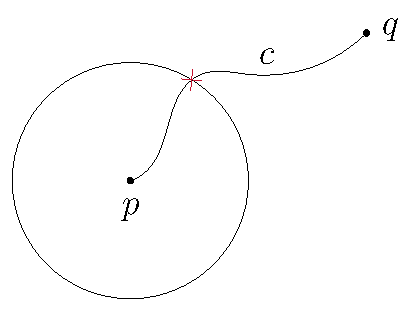
\includegraphics[scale=0.7]{figures/tikz/curvelength}
\end{minipage}


Wir erhalten damit:
\begin{align}
L(c) &\geq L(\eval{c}_{[a_0, b_0]})  \nonumber \\
&\geq L(\eval{c_v}_{[0, 1]}) = \norm{v}
\end{align}


mit Gleichheit wenn $c \equiv c_{[a_0, b_0]}$ eine Umparametrisierung von $\eval{c_v}_{[0, 1]}$ ist. Dies beweist Aussage $(1)$. Außerdem folgt aus $\norm{v} \geq \varepsilon$, falls $q\neq B_{\varepsilon}(p)$ die Aussage $(2)$.
\end{bew}
Mit diesem Wissen wollen wir nun den zuvor vorgestellten Satz beweisen.
\begin{bew}[Satz \ref{satz:metrischer_raum}]
Die ersten beiden Aussagen sind recht offensichtlich wahr.
\begin{itemize}
\item $\dd(p, q) \geq 0$ ist klar! 
\end{itemize}
\vspace{.1cm}
Es gilt $\dd(p, q)=0 \ \forall p \in \mfk$ für die konstante Kurve die Länge null hat. \\
Sei $\dd(p, q)=0$. Wir nehmen $p\neq q$ an. Wähle $r>0$, so dass $\eval{\expp_p}_{B_r(0)}$ ein Diffeomorphismus ist und betrachten $q \notin \expp_p(B_r(0))$. \\
Gemäß des Hilfslemmas hat jede Kurve von $p$ nach $q$ mindestens die Länge $r$. \\
Daraus folgt: 
\begin{align*}
\dd(p, q) > r > 0 \quad\text{\Large{\lightning}}
\end{align*}\
\begin{itemize}
\item $\dd(p, q) = \dd(q, p)$ ist ebenfalls klar! (Laufe die Kurve rückwärts ab)
\item \underline{Dreiecksungleichung}: 
\end{itemize}


\begin{minipage}[H]{0.99\textwidth}
Sei $\varepsilon>0$. Wähle $c_1$ und $c_2$ so, dass:
\begin{align*}
L(c_1) &\leq \dd(p, r) + \varepsilon \\
L(c_2) &\leq \dd(r, q) + \varepsilon
\end{align*}
\end{minipage}
\hspace{-3cm}
\begin{minipage}[H]{.3\textwidth}
\vspace{-1.7cm}
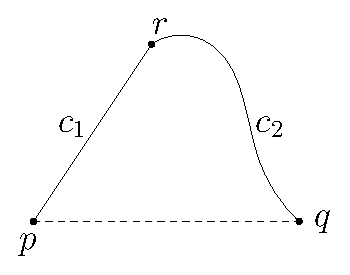
\includegraphics[scale=0.7]{figures/tikz/dreiecksungleichung}
\end{minipage} \\

Die Kurve $c = c_1 \star c_2$ sei nun diejenige Kurve, die durch $c_1$ und $c_2$ gegeben ist.
\begin{align*}
\dd(p, q) \leq L(c) &= L(c_1) + L(c_2) \\
&= \dd(p, r) + \dd(r, q) +2\varepsilon
\end{align*}
Dies zeigt für alle $\varepsilon>0$ die Dreiecksungleichung.
\begin{itemize}
\item Die Metrik induziert die ursprüngliche Topologie $(\mfk, \mathcal{T})$
\end{itemize}
Sei die Umgebung $U$ offen, das heißt $U \in \mathcal{T}$. Die Notation $U \ \text{offen}^d$ bedeutet offen bezüglich $d$. Wir wollen zeigen, dass $U \ \text{offen}^d$ impliziert, dass $U \in \mathcal{T}$. \\
Sei $U \ \text{offen}^d$, das heißt für jedes $p \in U \  \exists r(p)>0$, so dass $B_{r(p)} \subseteq U$. \\
Dann gilt:
\begin{align*}
B_{r(p)}(p)= \expp_p(B_{r(p)}(0))
\end{align*}
falls $r(p)$ \textbf{hinreichend klein} ist. Was dies genau bedeutet soll mit der Definition, die nach Beendigung des Beweises folgt geklärt werden. \\
Da $\expp_p$ ein Diffeomorphismus ist und $B_{r(p)(0)}$ offen, folgt:
\begin{align*}
&\Rightarrow B_{r(p)}(p) \ \text{ist offen} \\
&\Rightarrow U = \bigcup_{p \in U} B_{r(p)}(p) \ \text{ist offen}
\end{align*}
Die Umkehrung folgt sehr ähnlich und wird deshalb an dieser Stelle nicht vorgerechnet.
\end{bew} 
\begin{defs}[Injektivitätsradius]
Wir definieren den Injektivitätsradius in $p$ als: 
\begin{align}
\operatorname{injrad(p)} = \sup\{ r \ | \ \eval{\expp_p}_{B_r(0)}: B_r(0) \longrightarrow \expp_p(B_r(0)) \ \text{Diffeomorphismus}\}
\end{align}
\end{defs}
\begin{figure}[H]
	\centering
	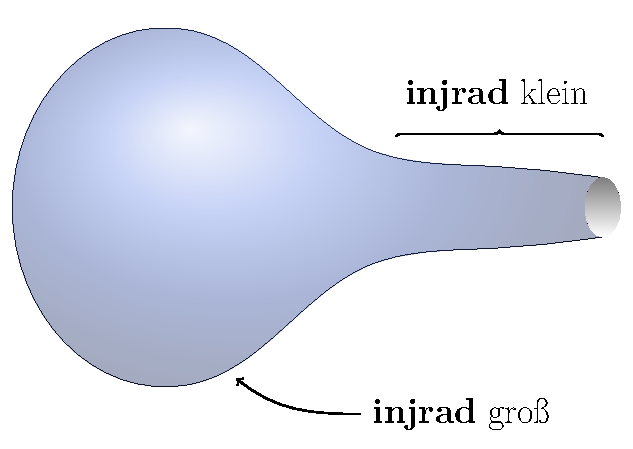
\includegraphics[scale=0.6]{figures/tikz/injrad}
	\caption{Darstellung der Bedeutung des Injektivitätsradius}
\end{figure}
Damit erhalten wir ein Kriterium für die im im Beweis des vorangegangenen Satzes verwendete Forderung nach "hinreichender Kleinheit":
\begin{align}
r(p) \ \text{hinreichend klein} \quad \Leftrightarrow \quad r(p) \leq \operatorname{injrad}(p)
\end{align}

\begin{lem}
$\dd$ ist stetig.
\end{lem}
\begin{bew}
Zunächst zeigen wir, dass $\dd(p,-)$ stetig in $p$ ist. \\
Sei $U \subset \mfk, V \subset T_p\mfk$ so, dass $\expp_p: V \longrightarrow U$ ein Diffeomorphismus ist. \\
Sei $p_n \in \mfk$ eine Folge mit $p_n \rightarrow p$. Dann gibt es $v_n \in T_p\mfk$ mit $v_n \rightarrow 0$ so, dass $\expp_p(v_n) = p_n$. Wir erhalten:
\begin{align*}
\dd(p, p_n) \leq \int_0^1 \norm{\dot{c}_{v_n}(t)} \dd t = \norm{v_n} \longrightarrow 0
\end{align*}
\end{bew}

\begin{itemize}
\item $\dd: \mfk \times \mfk \longrightarrow \R $ stetig.
\end{itemize}
Seien $p_n \rightarrow p$ und $q_n \rightarrow q$ Folgen in $\mfk$. Dann gilt:
\begin{align*}
\abs{\dd(p, q)- \dd(p_n, q_n)} \overset{(\star)}{\leq} \dd(p, p_n) + \dd(q, q_n) \longrightarrow 0.
\end{align*}
Die Abschätzung ($\star$) gilt da: $\dd(p, q) \leq \dd(p, p_n) + \dd(p_n,q_n) + \dd(q_n, q)$. 
